%! Author = joels
%! Date = 10/01/2022

\section{Beyond GoF}
\subsection{External Iterator}
\subsubsection{Problem}
\begin{itemize}
    \item Iteration through a collection depends on the target implementation
    \item Separate logic of iteration into an object to allow multiple iteration strategies
\end{itemize}
\textbf{Intent:}
\begin{itemize}
    \item How can strong coupling between iteration and collection be avoided, generalized and provided in a collection-optimized manner?
\end{itemize}
\subsubsection{Solution}
Provide a way to access the elements of an aggregate object sequentially without exposing its underlying representation.\\ 
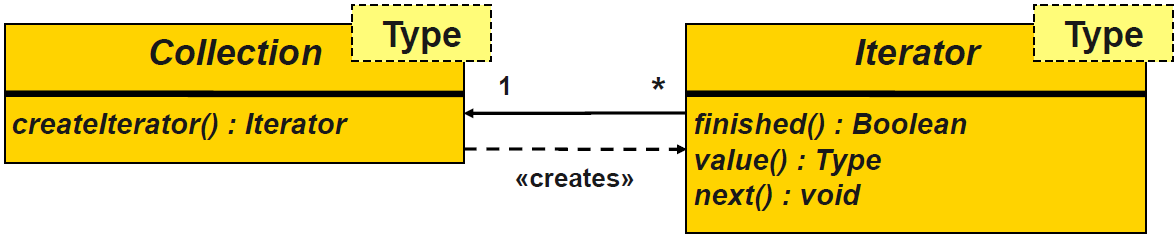
\includegraphics[width=\linewidth]{./img/external_iterator.png}
\textbf{Elementary operations of an Iterator's behaviour:}
\begin{itemize}
    \item Initializing an iteration \textit{new ArrayList().iterator();}
    \item Checking a completion condition \textit{it.hasNext();}
    \item Accessing a current target value \textit{var x = it.next();}
    \item Moving to the next target value \textit{it.next();}
\end{itemize}
\subsubsection{Summary}
\textbf{Benefits:}
\begin{itemize}
    \item Provides a single interface to loop though any kind of collection
\end{itemize}
\textbf{Liabilities:}
\begin{itemize}
    \item Multiple iterators may loop through a collection at the same time
    \item Life-Cycle Management of iterator objects
    \item Close coupling between Iterator and Collection class
    \item Indexing might be more intuitive for programmers
\end{itemize}

\subsection{Enumeration Method}
\subsubsection{Problem:}
\begin{itemize}
    \item Iteration management is performed by the collection's user
    \item Avoid state management between collection and iteration
\end{itemize}
\textbf{Intent:}
\begin{itemize}
    \item How can a collection be iterated considering the collection state and furthermore state management be reduced?
\end{itemize}
\subsubsection{Solution}
Support encapsulated iteration over a collection by placing responsibility for iteration in a method on the collection. The method takes a Command object that is applied to the elements of the collection.\\ 
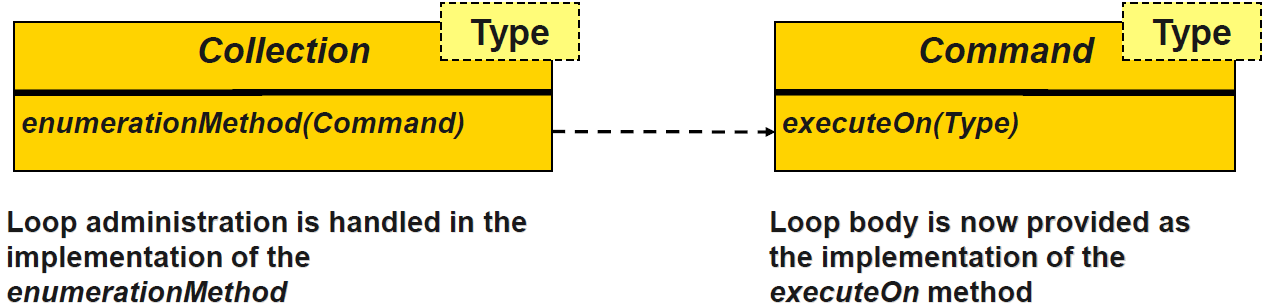
\includegraphics[width=\linewidth]{./img/enumeration_method.png}
\subsubsection{Summary}
Programming languages already implement Enumeration Method as their loop construct. (e.g. \textit{.forEach()})\\ 
\textbf{Benefits:}
\begin{itemize}
    \item Client is not responsible for loop housekeeping details
    \item Synchronization can be provided at the level of the whole traversal rather than for each element access
\end{itemize}
\textbf{Liabilities:}
\begin{itemize}
    \item Functional approach, more complex syntax needed
    \item Often considered too abstract for programmers
\end{itemize}

\subsection{Batch Method}
\subsubsection{Problem}
\begin{itemize}
    \item Collection and client (iterator user) are not on the same machine
    \item Operation invocations are no longer trivial
\end{itemize}
\textbf{Intent:}
\begin{itemize}
    \item How can a collection be iterated over multiple tiers without spending far more time in communication than in computation?
\end{itemize}
\subsubsection{Solution}
Group multiple collection accesses together to reduce the cost of multiple individual accesses in a distributed environment.
\begin{itemize}
    \item Define a data structure which groups interface calls on client side
    \item Provide an interface on servant to access groups of elements at once
\end{itemize}

\subsection{Objects for State}
\subsubsection{Problem}
\begin{itemize}
    \item Object's behaviour depends on its state, and it must change its behaviour at run-time
    \item Operations have large, multipart conditional statements (Flags) that depend on the state
\end{itemize}
\textbf{Intent:}
\begin{itemize}
    \item How can an object act according to its state without multipart conditional statements?
\end{itemize}
\subsubsection{Solution}
Allow an object to alter its behaviour when its internal state changes. The object will appear to change its class.\\ 
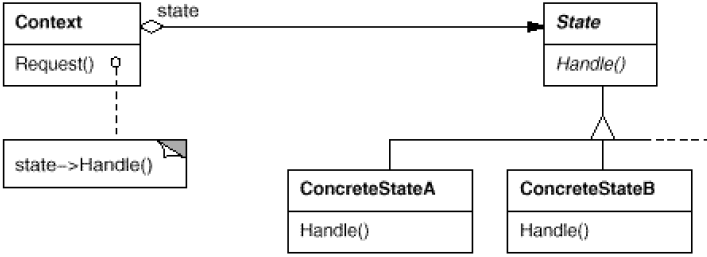
\includegraphics[width=\linewidth]{./img/objects_for_state.png}
\textbf{Dynamic:}\\
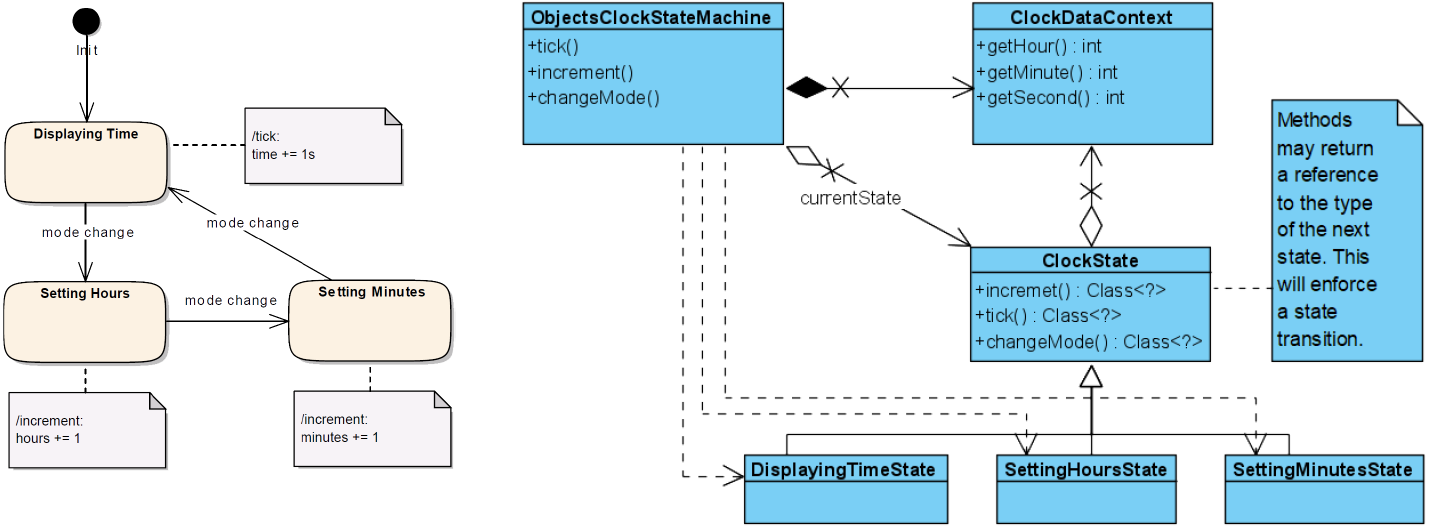
\includegraphics[width=\linewidth]{./img/objects_for_state_dynamic.png}
\subsubsection{Summary}
\textbf{Criticism:}
\begin{itemize}
    \item Complex, but does not adequately cover that complexity
    \item Overkill in many cases
    \item Name suggests problem domain rather than the solution
\end{itemize}

\subsection{Methods for State}
\subsubsection{Solution}
\begin{itemize}
    \item Each state represents a table or record of method references
    \item The methods reference lie on the State Machine (context) object
\end{itemize}
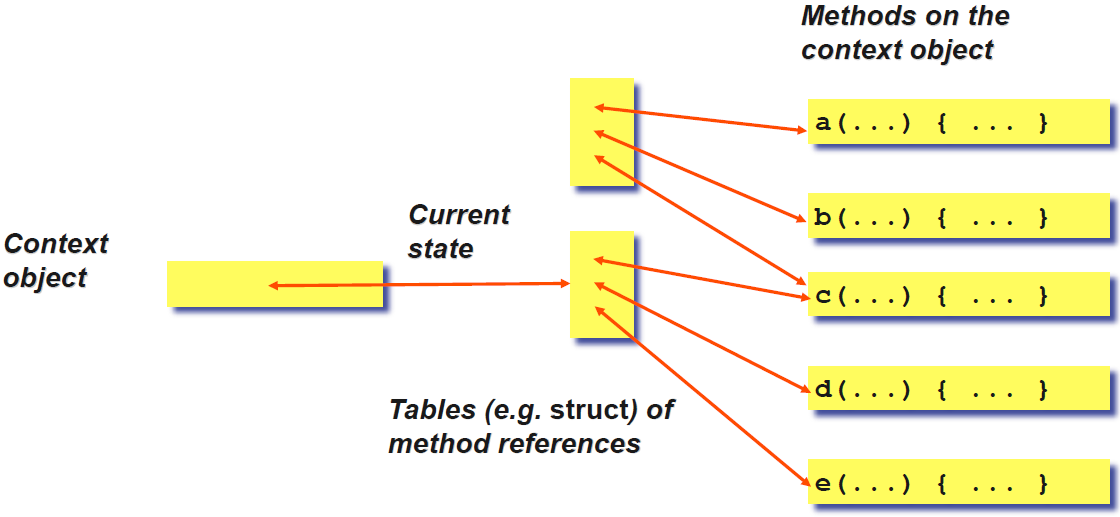
\includegraphics[width=\linewidth]{./img/method_for_state.png}
\textbf{Dynamics:}\\ 
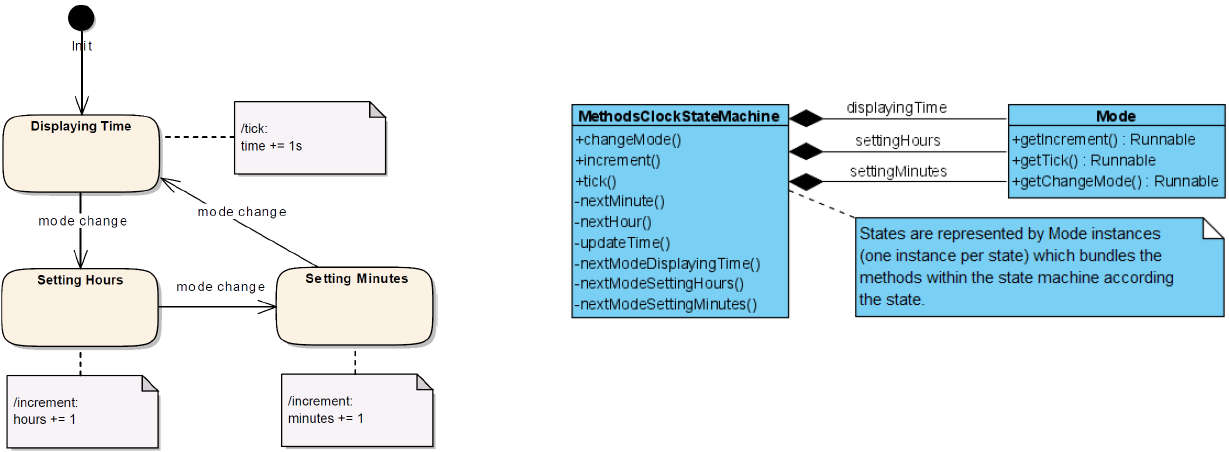
\includegraphics[width=\linewidth]{./img/method_for_state_dynamic.png}
\subsubsection{Summary}
\textbf{Benefits}
\begin{itemize}
    \item Allows classes to express different behaviours in ordinary methods themself
    \item Behaviour coupled to the state machine, not scattered accross small classes
    \item Each distinct behaviour is assigned its own method
    \item No object context needs to be passed around, methods can already access the internal stte of the State Machine
\end{itemize}
\textbf{Liabilities}
\begin{itemize}
    \item Requires an additional two levels of indirection to resolve a method call
    \item The state machine may end up far longer than was intended or is manageable
\end{itemize}

\subsection{Collection for State}
\subsubsection{Solution}
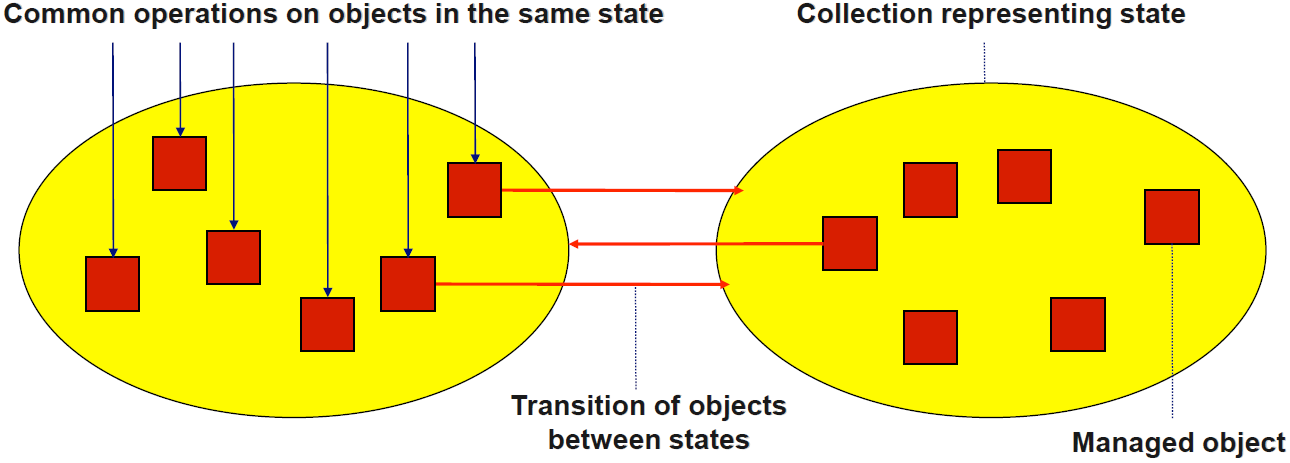
\includegraphics[width=\linewidth]{./img/collection_for_state.png}
\textbf{Dynamics:}\\ 
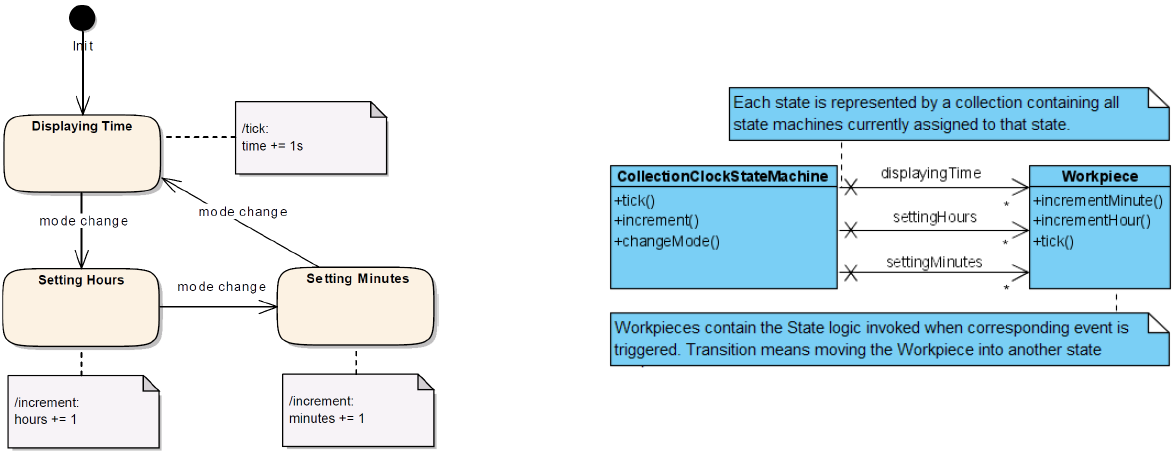
\includegraphics[width=\linewidth]{./img/collection_for_state_dynamic.png}
\subsubsection{Summary}
\textbf{Benefits:}
\begin{itemize}
    \item No need to create a class per state
    \item Optimized for multiple objects (state machines) in a state
    \item Object's collection implicitly determines its state
    \item Can be compined with other state machine (Objects / Methods)
\end{itemize}
\textbf{Liabilities:}
\begin{itemize}
    \item Can lead to a more complex state manager
\end{itemize}

\subsection{Implementation of State Patterns}
\textbf{Objects:} 
\begin{itemize}
    \item Results in a lot of classes and structures
    \item At least one class per state plus state machine
\end{itemize}
\textbf{Methods:}
\begin{itemize}
    \item Propagates a single class with a lot of methods
\end{itemize}
\textbf{Collection:}
\begin{itemize}
    \item Allows to manage multiple state machines with the same logic
    \item Splits logic and transaction management into two classes
\end{itemize}